\documentclass[11pt,a5paper]{article}
\usepackage[utf8]{inputenc}
\usepackage[english]{babel}
\usepackage{amsmath}
\usepackage{graphicx}
\usepackage{amsthm}
\usepackage{amsfonts}
\usepackage[margin=0.47in]{geometry}

\newtheorem{theorem}{}
\newtheorem{definition}{Definition}
\newtheorem{exercise}{Exercise}
\newtheorem{problem}{Problem}
\newtheorem*{corollary}{Corollary}

\title{\textbf{Sets and Infinity}}
\date{Week 3}
%\author{Miroslav Stankovic\\ Marko Puza}
\begin{document}
\maketitle




\section{Naive Set Theory}

The idea of infinity have always been part of mathematics and philosophy. It has been part of fameous Zeno's paradoxes, infinite lines in geometry, or basis of analysis in the times of Leibnitz and Newton. However, until late 18th century, the infinity was viewed as something indefinite - as a limit, towards which a variable goes.

\begin{definition}
By a \emph{set} we understand any collection into a whole $M$ of definite and separate objects $m$ of our intuition or our thought. These objects are called the \emph{elements} of $M$.
\end{definition}

\noindent The definition above was used by Georg Cantor to establish the foundations of set theory, which allowed, for the first time, to directly work with infinity. As you may notice, the Cantor's definition lack the precision and rigour we are used to. In 1901, Bertrand Russel came up with a paradox in the Cantor's set theory. It goes like this: $S=\{x|x\notin x\}$.

\begin{exercise} What is the Russel's paradox about?
\end{exercise}

\noindent Cantor's set theory was later 'fixed' using mathematical logic and rigorous axiomatic approach to study sets. For the time being, the naive set theory will be sufficient to demonstrate basic concepts in infinities.

\section{Infinities}

\noindent In set theory, Cantor's diagonal argument was published in 1891 as a mathematical proof that there are infinite sets which cannot be put into one-to-one correspondence with the infinite set of natural numbers. Such sets are now known as uncountable sets, and the size of infinite sets is now treated by the theory of cardinal numbers which Cantor began. 

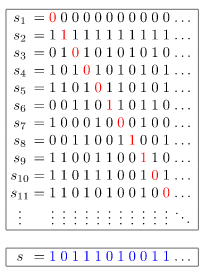
\includegraphics[scale=0.8]{cda}
\begin{exercise} Let $S=\{x|x\subset \mathbb{N}\}$. Show that there is no bijection from $\mathbb{N}$ to $S$.
\end{exercise}
\begin{corollary} There are infinities of different sizes.
\end{corollary}
\begin{problem} Can Cantor's diagonal argument be used to prove existence of sets bigger than $\mathbb{R}$?
\end{problem}

\subsection*{Comparing infinities}

\noindent So how to compare two infinite sets? We can try to pair the elements, and if we are successful the sets are same size; if some elements are left umpired in a set, that set is bigger. Based on this idea we use following definition:

\begin{definition}
$A\preceq B$ if there is an injective function from $A$ to $B$;

$A\approx B$ if there is a bijection from $A$ to $B$; 

$A\prec B$ if $A\preceq B$ and $A\not\approx B$.
\end{definition}


\noindent There are several obvious properties of $\preceq, \approx, \prec$.
\begin{enumerate}
  \item $A\approx A$
  \item $A\approx B \Rightarrow B\approx A$
  \item If $A\approx B$ and $B\approx C$ then $A\approx C$
  \item If $A\preceq B$ and $B\preceq C$ then $A\preceq C$
  \item If $A\approx B$ then $A\preceq B$ and $B\preceq A$
\end{enumerate}

\noindent You might be surprised, that following (very plausible) property is missing: $A\preceq B$ and $B\preceq A$ then $A\approx B$. Even though it is true, it is not at all obvious! This theorem is known as Cantor-Bernstein theorem.

\begin{problem} Prove the Cantor-Bernstein theorem.
\end{problem}

\begin{exercise} Show that $(0,1)\approx\mathbb{R}$.
\end{exercise}

\subsection*{Finite vs. infinite}

\noindent Let's look at the following properties of finite sets.
\begin{enumerate}
  \item If $A$ is finite and $a \not\in A$ then $A\prec (A\cup \{a\})$.
  \item If $A$ is finite and $B\subset A$ then $B\prec A$.
  \item If $A$ is finite with at least two elements then $A \prec A\times A$ .
\end{enumerate}

\noindent However, none of these 'obvious' statements are true for infinite sets. Take $A\approx \mathbb{N}$. Then $\mathbb{N} \approx \mathbb{N}\cup \{0\}$ - we can take bijection $f(x) = x+1$. If $B$ is set of even natural numbers, then $B\subset A$ but $B\approx A$ thanks to bijection $f(x) = x/2$. And finaly:
\begin{exercise}
Show that $\mathbb{N} \approx \mathbb{N} \times \mathbb{N}$.
\end{exercise}

\noindent So even if cartesian product creates, in some sense, much bigger set, it is still the same countable infinity. In fact, $A\approx A\times A$ for any infinite set $A$. As a consequence, $A\approx A^n$ for any $n\in \mathbb{N}$. Another way how to create 'bigger' sets is using union - and since today it is all about infinity, let it be infinite union!
\begin{theorem}
Countable union of countable sets is countable.
\end{theorem}
\begin{proof} Consider the countable sets $S_0, S_1, S_2, \ldots$ where $\displaystyle S = \bigcup_{i \mathop \in \mathbb{N}} {S_i}$. Now we write the elements of $S_0, S_1, S_2, \ldots$ in the form of a table:

$\begin{array} {*{4}c} {a_{00}} & {a_{01}} & {a_{02}} & \cdots \\ {a_{10}} & {a_{11}} & {a_{12}} & \cdots \\ {a_{20}} & {a_{21}} & {a_{22}} & \cdots \\ \vdots & \vdots & \vdots & \ddots \\ \end{array}$

\noindent where $a_{ij}$ is the $j$th element of set $S_i$. This table clearly contains all the elements of $\displaystyle S = \bigcup_{i \mathop \in \mathbb{N}} {S_i}$, so we have $S \approx \mathbb{N}\times\mathbb{N} \approx \mathbb{N}$.
\end{proof}

\begin{exercise} Using Cantor-Bernstein theorem, show that $\mathbb{Q}\approx\mathbb{N}$. 
\end{exercise}
\begin{problem} Show that $\mathbb{R} \approx \mathbb{N} \times \mathbb{R}$.
\end{problem}
\begin{problem} Show that $\mathbb{R} \approx \mathbb{R} \times \mathbb{R}$.
\end{problem}
\begin{problem} Show that set of all finite subsets of $\mathbb{N}$ is countable.
\end{problem}


\end{document}
\\https://mks.mff.cuni.cz/common/show.php?title=Nekone%26%23269%3Bn%26eacute%3B+mno%26%23382%3Biny&file=library/NekonecneMnozinyDS/NekonecneMnozinyDS
\\https://mks.mff.cuni.cz/common/show.php?title=Teorie+mno%26%23382%3Bin&file=library/TeorieMnozinPPo/TeorieMnozinPPo
\\https://en.wikipedia.org/wiki/Cantor%27s_diagonal_argument
\\https://mks.mff.cuni.cz/library/AGNerovnostLZ/AGNerovnostLZ.pdf
